\section{Lecture 13: Quantum Harmonic Oscillator}

Consider a classical oscillator. 

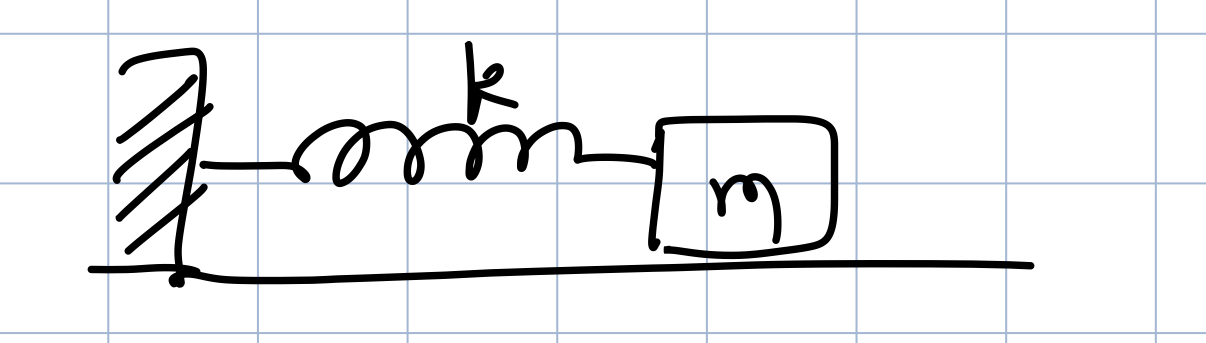
\includegraphics[width=300px]{spring.jpeg}

We know
\[ \mbf{F} = - k \mbf{x}, V(x) = \frac{1}{2} kx^2 = \frac{1}{2} m \omega^2 x^2 \]

where $\omega = \sqrt{\frac{k}{m}}$. The potential looks like

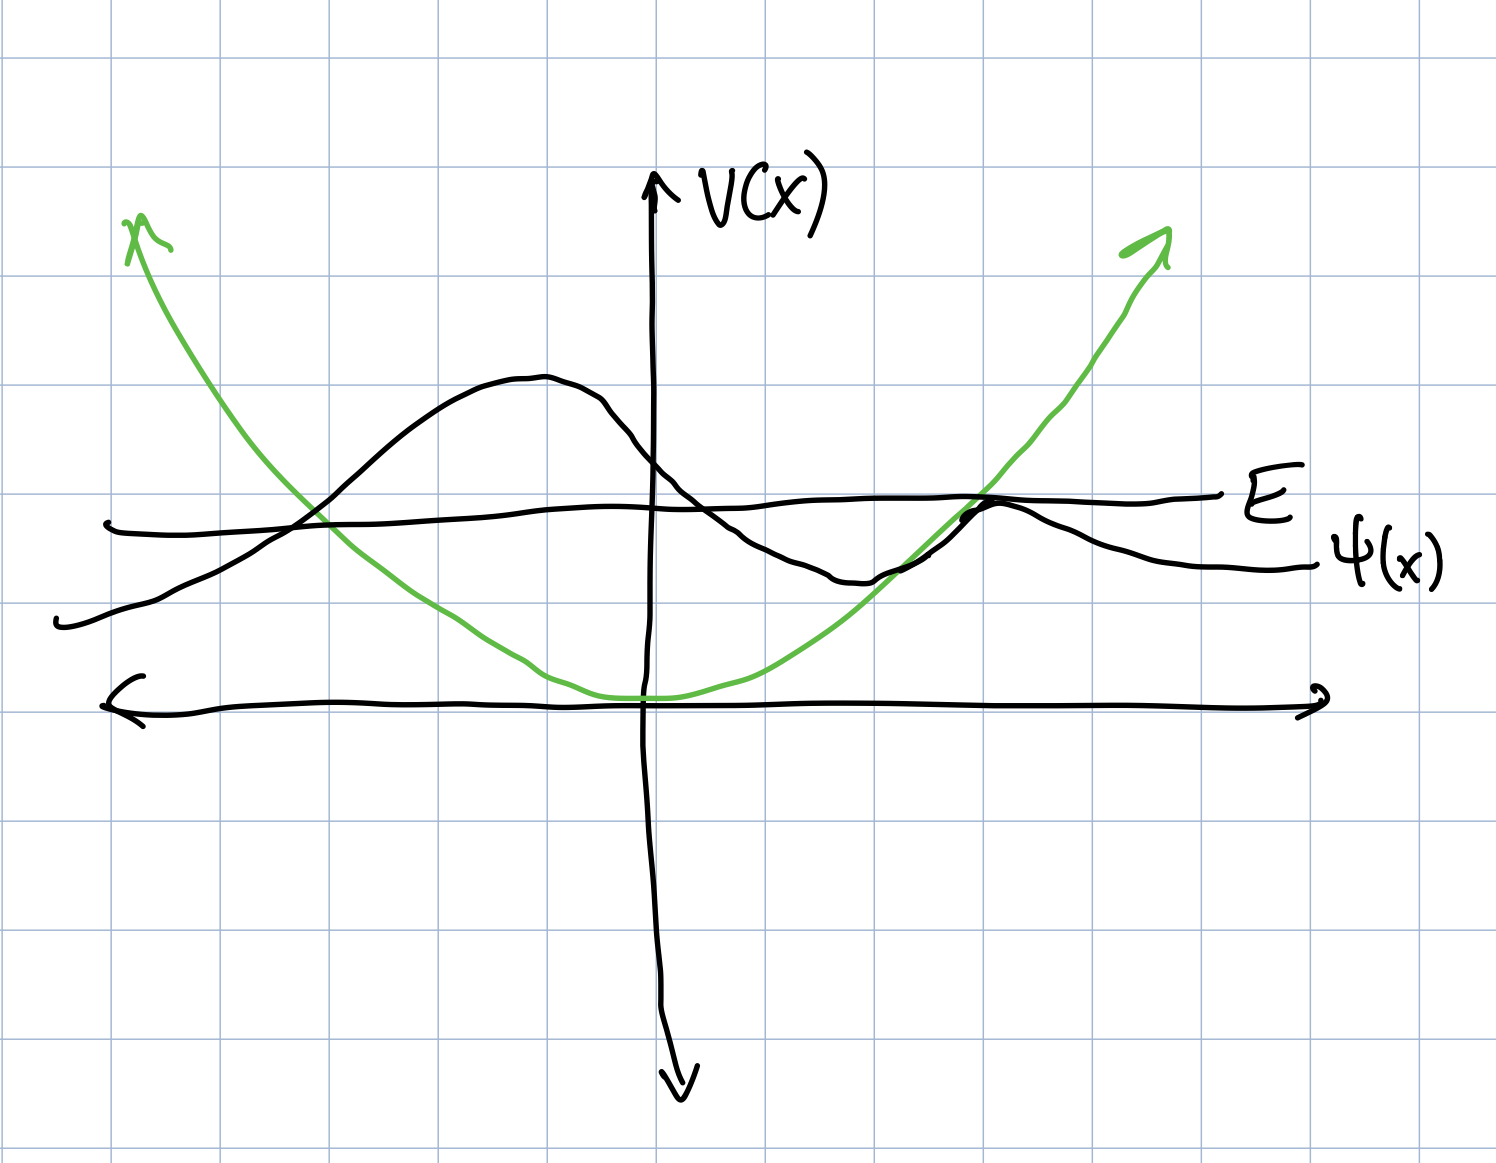
\includegraphics[width=300px]{springpot.jpeg}

The time-independent Schrodinger equation looks like:
\[ -\frac{\hbar^2}{2m} \derivative{^2 \Psi}{x^2} + \frac{1}{2} kx^2 \Psi = E \Psi \]
Let's go to dimensionless variables to make our lives easier. Let $\lambda = \frac{2E}{\hbar \omega}$ (a redimensioned energy),
$\xi = \qty(\frac{m \omega}{\hbar})^{1/2} x$, so:
\[ \derivative{^2}{\xi^2} \Psi(\xi) + (\lambda - \xi^2) \Psi(\xi) = 0 \]
we are going to consider the asymptotic solution for large values of $\xi \gg \lambda$.
\[  \qty(\derivative{^2}{\xi^2} - \xi^2) \Psi(\xi) = 0 \]
The solution to this is $\Psi(\xi) = e^{\pm \xi^2/2}$, but we want something
that doesn't bother you at large arguments
and applying normalization (boundary conditions at infinity must be 0), $\Psi(\xi) \approx \xi^p e^{-\xi^2/2}$ for some power $p$.
More generally,
\[ \Psi(\xi) = e^{-\xi^2/2} H(\xi) \]
for some function $H$ which respects the asymptotic behavior at large arguments. Substituting
our candidate back in, we get:
\begin{align*}
    \derivative{^2H}{\xi^2} - 2 \xi \derivative{H}{\xi} + (\lambda - 1)H &= 0
\end{align*}
This is a well-studied equation called the Hermite equation. The solutions for $H$ are called the Hermite polynomials.
Let's solve by power-series expansion. Since the parity of $\Psi(x)$ is definite
for a symmetric potential and the Gaussian is even, $H(\xi)$ must also have definite parity.
First look at the even solutions
\[ H(\xi) = \sum_{\ell = 0}^{\infty} c_{\ell} \xi^{2\ell} \]
where $c_0 \neq 0$. Substituting into the equation, we have:
\begin{align*}
    \sum_{\ell = 0}^{\infty} \qty[(2 \ell)(2 \ell - 1) c_{\ell} \xi^{2(\ell - 1)} + (\lambda - 1 - 4\ell) c_{\ell}\xi^{2\ell}] &= 0 \\
    \sum_{\ell = 0}^{\infty} \qty[2(\ell + 1)(2 \ell + 1) c_{\ell + 1} + (\lambda - 1 - 4\ell) c_{\ell}]\xi^{2\ell} &= 0 \\
    2(\ell + 1)(2 \ell + 1) c_{\ell + 1} + (\lambda - 1 - 4\ell) c_{\ell} &= 0 \\
    c_{\ell + 1} = \frac{(4\ell + 1 - \lambda)}{2(\ell + 1)(2 \ell + 1)} c_{\ell}
\end{align*}
But we still need $c_0$ and we are unsure if this series even converges. By the ratio test, let's look at:
\[ \lim_{\ell \to \infty} \frac{c_{\ell + 1}}{c_{\ell}} = \lim_{\ell \to \infty } \frac{(4\ell + 1 - \lambda)}{2(\ell + 1)(2 \ell + 1)} \sim \frac{1}{\ell} \]
What if $H$ were an exponential? Then:
\begin{align*}
    e^{\xi^2} = \sum_{\ell} \frac{\qty(\xi^2)^{\ell}}{\ell!} \implies \frac{c_{\ell + 1}}{c_{\ell}} = \frac{1}{\ell}
\end{align*}
But this would diverge the wave function! $\Psi \sim e^{\xi^2} \xi^p e^{-\xi^2/2}$
so $\Psi \sim \xi^p e^{\xi^2/2}$ which is non-normalizable. Let the highest power be $\xi^{2N}$ where $N = 0, 1, 2, \dots$.
This means $c_N \neq 0$ but $c_{N + 1} = 0$, which means the rest of the terms are 0. This means:
\[ 4(N + 1) + 1 - \lambda = 0 \implies \lambda = 4N + 1\]
$\lambda = 1, 5, 9, \dots$, so energy is quantized!

For the odd solution, we could do exactly the same thing, just for the odd power series instead. Here is the flow:
\begin{enumerate}
    \item Make a power series: $d_0 \neq 0$
    \[ \sum_{\ell = 0}^{\infty} d_{\ell} \xi^{2\ell + 1} \]
    \item Find a recurrence relation:
    \[ d_{\ell + 1} = \frac{4 \ell + 3 - \lambda}{2(\ell + 1)(2 \ell + 3)} \]
    \item Solve for
    \[ \lambda = 4N + 3, \lambda = 3, 7, 11, \dots \]
\end{enumerate}
Together, $\lambda$ can quantized be any odd nautral. So for any $n = 0, 1, 2, \dots$:
\[ E_n = \qty(n + \frac{1}{2}) \hbar \omega \]

Let's take a look at the energy spectrum.

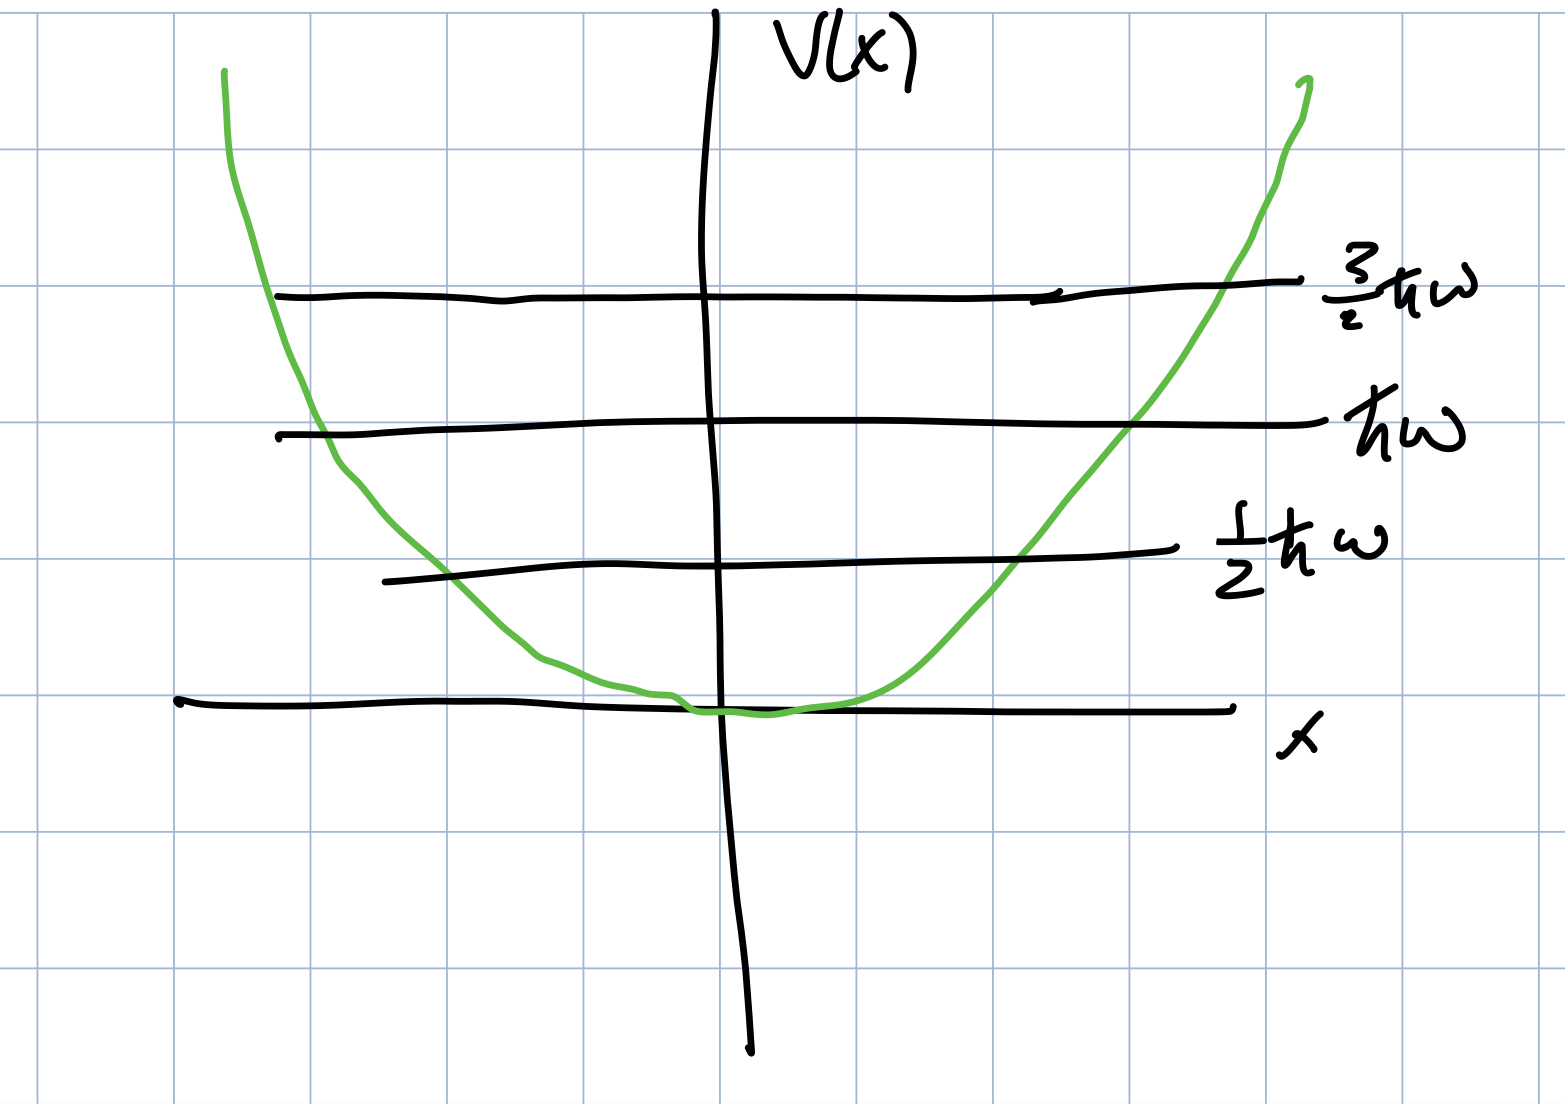
\includegraphics[width=300px]{qhmnrg.jpeg}

Note that the minimum energy is not 0, this would violate Heisenberg Uncertainty Principle.
In fact, any oscillatory mode must have some minimum energy. The vacuum has some
(tiny) energy always! This is called ``zero-point motion''.

Furthermore, the levels are equally spaced.